\renewcommand{\thesection}{\Roman{section}}
\section{Methods}

\subsection*{System}

\quad The system we will use to conduct our experiments consists of the 7-DOF Barrett WAM robot arm and 4-DOF Barrett BH-280 Hand from Barrett Technology, Inc. The robot is equipped with one 6-DOF wrist torque sensor, three 1-DOF finger joint torque sensors, and four 24-DOF tactile pressure sensors, making for a total of 105 independent sensor inputs. Given such rich sensory input, we hope to invent feature vectors which exhibit statistically significant differences between different grasp shapes. Such a feature vector could be used to augment the grasp preshaping algorithm of Humberston and Pai \cite{Ben}.

All the sensors described above read at 125\,Hz. Most afferent inputs in humans run at less than 60\,Hz, so this rate is enough for any biologically motivated algorithms we decide to implement \cite{Howe}.

\subsection*{Experimental Setup}

\quad We will begin the project with a basic implementation and an experiment. First, we will implement a robotic controller which mirrors the adaptive grasp shaping algorithm of [ben] as closely as possible. When complete, we will use this controller to conduct some simple grasp and lift experiments with simple, known objects.
\begin{figure}[H]
%\begin{minipage}{17cm}
	\centering
	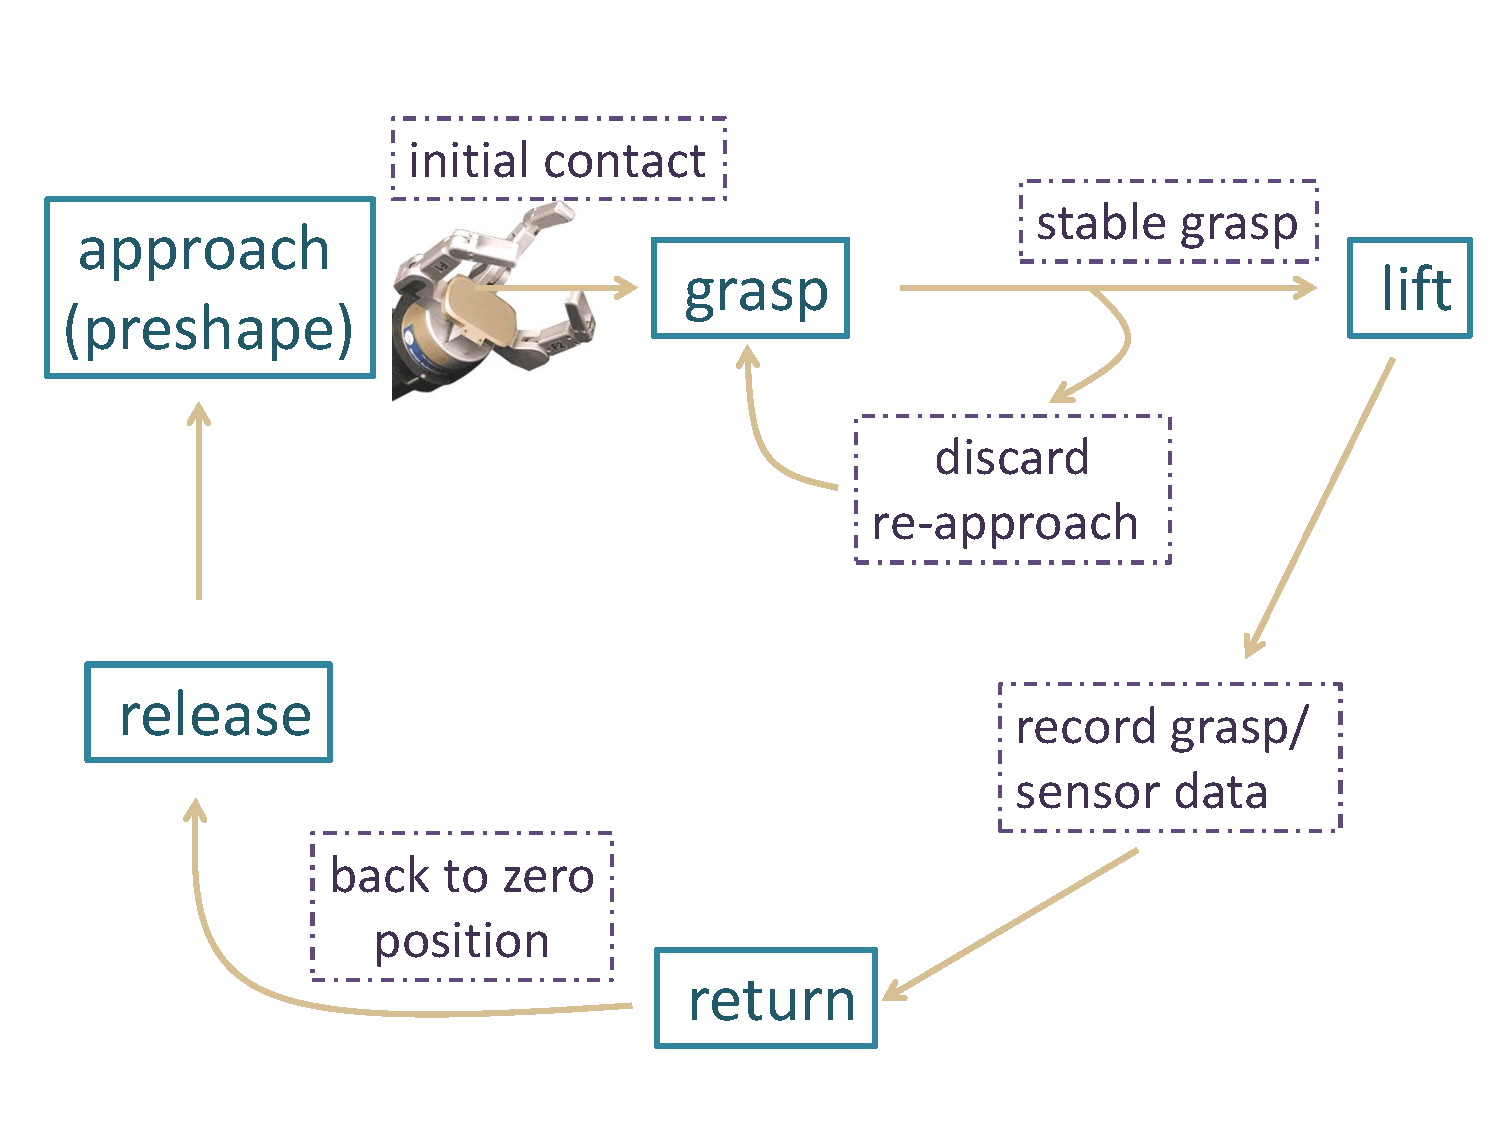
\includegraphics[width=0.5\textwidth]{programStructure.pdf}	
	%\setlength{\captionmargin}{50pt}
	\caption{Overview of experimental succession. Bold solid boxes indicate the active 
phases of the Barrett hand, while dashed boxes represent the grasp adaptation mechanisms.}
	\label{workflow}
%\end{minipage}
\end{figure}
The basic workflow of our project is as follows (see also Figure \ref{workflow}):
\begin{enumerate}
\item Approach the object from a nearby location (possibly by a pre-recorded trajectory).
\item When close to the object (or when contact is detected), close the hand's fingers. Possibly iterate this step a few times.
\item When the fingers stop closing or contact is detected, slowly lift upward.
\item Stop when some predetermined height is reached.
\item Return to table height and release the grip on the object.
\end{enumerate}

Sensor data will be recorded throughout this process, but especially in steps 2 and 4. This will give us a good picture of what sensor readout is like (1) when contact is first established and (2) during a stable grasp.

After performing this experiment and collecting substantial sensor data, we will analyze the data to determine our next course of action. See the Future Work section for a discussion of some possibilities.

\subsection*{Difficulties and Limitations}

\quad The Barrett Hand only has 4 degrees of freedom: one rotational axis of motion for each of the three fingers, plus the angle of the two outer fingers. Though each finger has two joints, these joints cannot be controlled directly by software using the libbarrett API; instead, the second joint is automatically controlled by a "torque switch" algorithm \cite{manual} . This limits our ability to preshape grasps: our shapes will consist only of these 4 DOFs and will not match the shapes we sample while lifting an object. Nevertheless we believe it will be worthwhile to apply preshaping to the task of manipulation with the Barrett.

Ben Humberston has made significant progress in the area of adaptive grasp shaping, but we cannot use much of his specific algorithms. Our methods must be significantly different because we do not have the luxury of working in a virtual environment where we can place fingers at arbitrary locations within the grasp frame. Instead, given some target grasp shape, we must use forward kinematics to calculate the necessary joint angles to achieve such a grasp. As a result, our definition of grasp shape will necessarily be very different.

Another difference between Humberston's work and ours is that his is a human-in-the-loop system. Essentially, the human performs the work of "controller" under his experimental setup. In our setup, the robot must be autonomous. We can alleviate some of the difficulty by executing motions that were pre-recorded by a human. The libbarrett example code includes a "Teach and Play" system that makes it easy to teach the robot such predefined movements.

Still, we will have to program a custom controller for much of the grasping task. For this, we intend to use a state machine, as has been successful in much of the past grasping research \cite{Leoni} \cite{Sikka}.
